\documentclass[russian, unicode, xcolor={dvipsnames}, aspectratio=43]{beamer}
% handout - to disable overlays
% handout - to disable overlays
\usepackage[russian]{babel}


\usepackage[T2A]{fontenc}
\usepackage[utf8]{inputenc}
\usepackage[russian]{babel}
\usepackage{hyphenat}
\hyphenation{три-го-но-мет-ри-чес-ких}

\usepackage{amsmath}
\usepackage{amssymb}
\usepackage{gensymb}

\usepackage{hyperref}
\hypersetup{
	colorlinks=true,
	%urlcolor=cyan
}




\usepackage{booktabs}
\usepackage{caption}
\captionsetup[table]{name=Таблица}
\usepackage{multirow}
\usepackage{csvsimple}
\usepackage{color, colortbl}	
\definecolor{Gray}{gray}{0.9}

\usepackage{graphics}
\usepackage{pgfplots}
\usepackage[listings,theorems]{tcolorbox}


\DeclareMathOperator{\re}{Re}
\DeclareMathOperator{\im}{Im}
\newcommand{\eqdef}{\stackrel{\mathrm{def}}{=}}
\newcommand{\ton}[1]{1, 2, \dots, #1}
\newcommand{\dd}[2]{\dfrac{\partial #1}{\partial #2}}

\newcommand{\adv}[1]{\textcolor{ForestGreen}{#1}}
\newcommand{\dis}[1]{\textcolor{Maroon}{#1}}

\definecolor{optargs}{rgb}{0.49, 0.56, 0.16}
\usetheme{metropolis}
\title{Практикум по компьютерным технологиям}
\author{Преподаватель: Егор Павлович Фадеев}
\institute{МГУ $\bullet$ Физический факультет $\bullet$ Кафедра математического моделирования и информатики}
\date{\today}




\begin{document}

\maketitle
	
\begin{frame}{О курсе}
	\begin{tcolorbox}[colback=red!5,colframe=red!75!black,title=Требование к студенту]
		Наличие \textbf{ноутбука} и возможность носить его на занятия.
	\end{tcolorbox}
	
	\begin{tcolorbox}[colback=black!5,colframe=violet!45!black,title=О чём курс]
		\begin{itemize}
			\item[\adv{\checkmark}] \textbf{Python};
			\item[\adv{\checkmark}] Математическое моделирование;
			\item[\adv{\checkmark}] Научные библиотеки;
			\item[\adv{\checkmark}] \textbf{\LaTeX};
			\item[\dis{$\times$}] Web разработка и т.п.
		\end{itemize}
	\end{tcolorbox}
	
		
\end{frame}

\begin{frame}{Программа курса. Осень}
	
	\begin{minipage}{0.49\textwidth}
		\textbf{Python}:
		\begin{itemize}
			\item Синтаксис;
			\item $\ldots$;
			\item Элементы ООП.  
		\end{itemize}
			
		\textbf{Библиотеки}:
		\begin{enumerate}
			\item \adv{NumPy} --- массивы чисел;
			\item \adv{matplotlib} --- визуализация данных и построение графиков;
			\item \adv{pandas} --- табличные данные. 
		\end{enumerate}
			

		
	\end{minipage}
	\begin{minipage}{0.49\textwidth}
		
		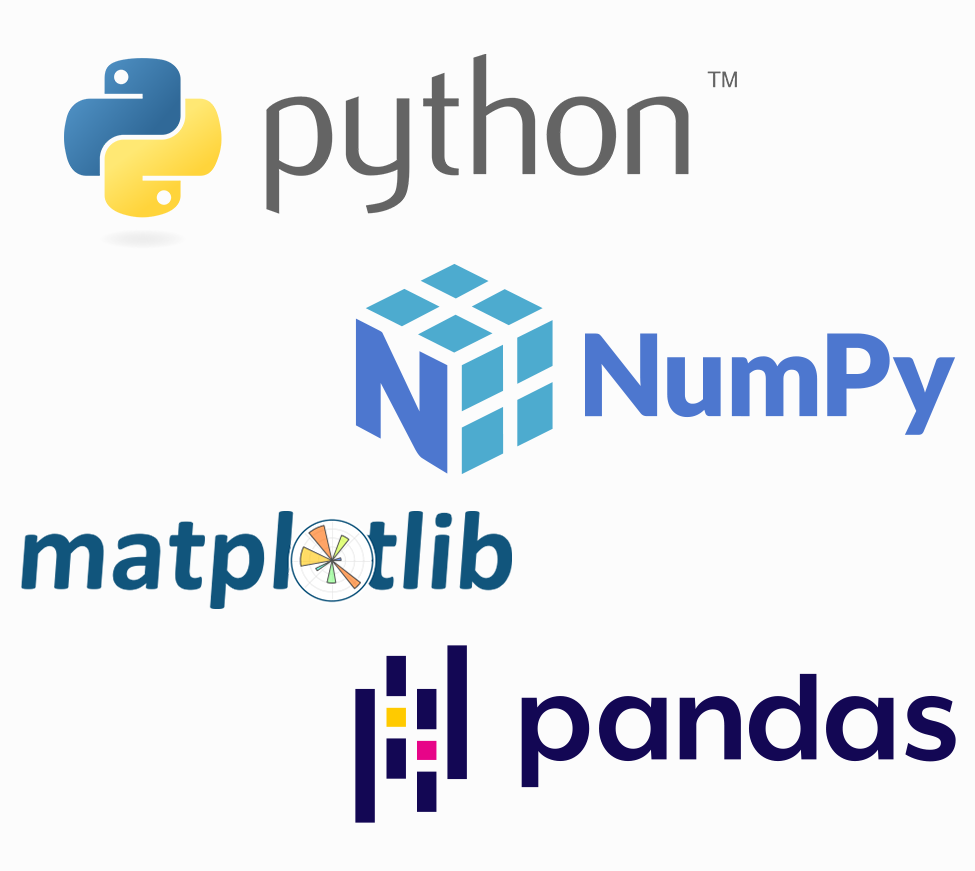
\includegraphics[width=0.9\textwidth]{pictures/autumn_logos.png}
		
		\begin{tcolorbox}[colback=green!5,colframe=green!75!black,title=Аттестация]
		6 домашних заданий.
		
		\textbf{Зачет}.	
		\end{tcolorbox}
		
		
	\end{minipage}
\end{frame}

\begin{frame}{Программа курса. Весна}
	
	\begin{minipage}{0.49\textwidth}
		Система верстки \LaTeX
		
		\textbf{Библиотеки:}
		\begin{enumerate}
			\item \adv{SciPy} --- научные вычисления;
			\item \adv{Qt} --- графический интерфейс;
			\item \adv{scikit-learn} --- классический ML;
			\item \adv{openCV} --- классическое CV;
			\item \adv{PyTorch} --- нейронные сети; 
		\end{enumerate}
	\end{minipage}
	\begin{minipage}{0.49\textwidth}
		
\includegraphics[width=0.9\textwidth]{pictures/spring_logos.png}
		
		\begin{tcolorbox}[colback=green!5,colframe=green!75!black,title=Аттестация]
			Домашнее задание по \textbf{математическому моделированию}.
			
			Домашнее задание по \textbf{\LaTeX}.
			
			Курсовая работа.
			
			\textbf{Зачет}.	
		\end{tcolorbox}
		
	\end{minipage}

\end{frame}



\end{document}
